% !TEX TS-program = xelatex
% !TEX encoding = UTF-8 Unicode

\providecommand{\home}{../..}
\documentclass[\home/main.tex]{subfiles}

\begin{document}

\chapter{Introduction, Setting and Background}\label{background:setting-and-background}

\Acrfull{WMS} is a measurement technique where\-by gas properties such as gas concentration and temperature can be extracted from light-matter interaction. The drive current (or temperature) of the laser diode is modulated with a sine signal around its bias value. This sine modulation will then cause a sine modulation of the emitted wavelength as well. Usually, the emitted power will also vary sinusoidally, but this modulation is not of interest in this measurement technique. This laser line interacts with the gasses present in the environment. The gas of interest should have a gas absorption peak within the wavelength range of this laser device. This absorption peak is also wavelength dependent and will result in non-linear transmission function, creating higher order harmonics of this sine wave at the detecting photodiode. The resulting light is incident on a photodiode. Using signal processing techniques, gas characteristics can be extracted. The construction of such a system forms the main goal of this dissertation. 

In this chapter, we will highlight the typical components of a wavelength modulation spectroscopy system, their function and trade-offs in such a system. First, we will discuss the relevance of measuring gas concentration and more specifically, \acrfull{CO} and \acrfullpl{CO2}. Next, we will compare different techniques that can be employed to measure gas concentrations and finally we will give a high-level overview of the measurement principles.

\section{Importance of Gas Concentration Measurements}

  Gas concentration measurements have applications in various domains such as air quality, food packaging, agriculture and human health. These applications are strongly gas dependent. In this dissertation, we focus on \acrshort{CO} and \acrshortpl{CO2} as gasses of interest.
  
  \acrshort{CO2} gas sensing can be applied to monitor the ambient air quality. By means of such a measurement, ventilation can be turned on or windows opened if the \acrshort{CO2} concentration exceeds a certain level. Outdoor \acrshort{CO2} monitoring is also possible for instance in the vicinity of coal plants and other industrial operations that produce large amounts of \acrshort{CO2}. 
  %http://www.sciencedirect.com/science/article/pii/S0925400599004116
  
  Another application domain is greenhouse crop production. Increased levels of CO\textsubscript{2} can improve photosynthesis and improve crop growth. The optimal levels of CO\textsubscript{2} are crop dependent, thus precise control is needed using accurate measurements \cite{nederhoff1994effects}.
  
  Modified atmospheres are often used in food packaging to preserve food longer. \acrshort{O2} concentrations are lowered while the concentration of \acrshort{CO2} is increased. An optical measurement can be used to verify package seal integrity. Another use of this measurement is to detect spoilage when higher than expected \acrshort{CO2} concentrations are detected \cite{CO2-food-preservation,CO2-food-sensors}.
  
  \begin{figure}
  	\centering
  	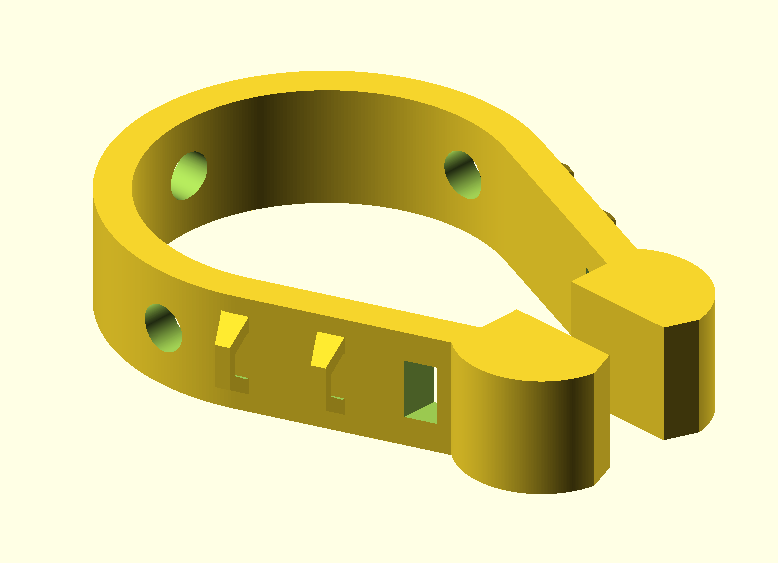
\includegraphics[width=0.3\linewidth]{\home/chapters/background/figures/clip}
  	\caption{This is a margin figure. The helix is defined by $x = \cos(2\pi z)$, $y = \sin(2\pi z)$, and $z = [0, 2.7]$. The figure was drawn using Asymptote}
  	\label{fig:clip}
  \end{figure}
  
  \acrshort{CO} is a poisonous gas for humans. \acrshort{CO} monitoring in rooms with potentially dangerous levels is important to alert people and activate ventilation if necessary. 

\section{Tuneable Diode Laser Absorption Spectroscopy}

  \Acrfull{WMS} is a well established technique for gas sensing and a special form of \acrfull{TDLAS}. By means of \acrshort{TDLAS}, gas properties such as concentration, temperature and flow rate can be determined \cite{WMSTemperature,TDLASVelocity,OpticalGasSensingReview}.

  In \acrshort{TDLAS}, the frequency (wavelength) of a laser is tuned by changing one of its input variables. Typical tuning factors are temperature and input current. By means of this variable wavelength, we can scan across one (or more) absorption peaks. Absorption peaks are wavelength dependent phenomena observed a gas' spectrum. A laser is biased such that it emits light in the neighbourhood of this peak and by changing the input variables, the entire peak is scanned. Based on the amount of incident power on a photo diode versus the emitted power, gas properties (concentration, temperature, mass flux\ldots) can be extracted with high accuracy \cite{OpticalGasSensingReview}. In this dissertation, we will only focus on measuring the gas concentration.

  The operating principle of \acrshort{TDLAS} is straightforward. By means of the Beer-Lambert law, that quantifies the amount of light absorbed by the transmission medium, the transmitted power can be related to concentration:
  \begin{equation}
    I(\nu) = I_0 \exp(-\alpha(\nu)L)
    \label{background:Beer-Lambert-law}
  \end{equation}

  The incident light intensity $I_0$ is transmitted through a gas cell of length $L$ (the length over which the light interacts with the gas) and absorbance $\alpha(\nu)$ with $\nu$ the wavenumber ($1/\lambda$). It is also assumed that the source is monochromatic (i.e.\ its optical bandwidth is much smaller than the bandwidth of the absorption lines) and that there are no chemical changes in the gas cell \cite{abs-spec-status-and-potential}. The absorbance $\alpha(\nu)$ can be written as \cite{RiekerDissertation}:% (e.g.\ dimer formation can cause deviations).
  \begin{equation}
    \alpha(\nu) = \sum_j S_j(T) P_i \phi_j(\nu-\nu_0)
    %\alpha = C_\text{mol}S\dfrac{\gamma}{\pi(\gamma^2 + (\nu-\nu_0)^2}
    \label{background:absorption-coefficient}
  \end{equation}

  where $S_j(T)$ is the line strength (in \si{\centi\metre^{-1}}) of absorbance feature $j$, $P_i$ the partial pressure (dimensionless) of the gas of interest and $\phi(\nu)$ the line shape profile (dimensionless and normalised to have unit amplitude at $\nu=0$). There are three line shape profiles: Lorentzian, Gaussian and Voigt. Equations~\ref{background:lorentzian},~\ref{background:gaussian} and~\ref{background:voigt}
  are the normalised line shapes ($*$~represents the continuous convolution) for the profiles.
    
%  \begin{subequations}
%  \label{background:line_shapes}
%  \begin{align}
%    \text{Lorentzian profile} &\qquad & \phi_L(\nu; \gamma) &= \dfrac{\gamma}{\pi\br{\gamma^2+\br{\nu-\nu_0}^2}} \label{background:lorentzian}\\
%    \text{Gaussian profile}  &       & \phi_G(\nu; \gamma) &= \sqrt{\dfrac{\ln{2}}{\pi}}\exp\br{-\ln{2}\br{\dfrac{\nu-\nu_0}{\gamma}}^2} \label{background:gaussian}\\
%    \text{Voigt profile}     &       & \phi_V(\nu)           &= \phi_L(\nu; \gamma_L) * \phi_G(\nu; \gamma_V) \label{background:voigt}
%  \end{align}
%  \end{subequations}
   
  Important parameters of these line shapes are line width and line strength (maximal amplitude). The width is usually described in terms of the \acrfull{HWHM} ($\gamma$) or \acrfull{FWHM} ($2\gamma$). The appropriate line shape depends on which of the broadening mechanisms dominate.
  
  A Lorentzian line shape is the result of lifetime/pressure broadening. Different molecular states have different lifetimes associated with them. Changes occur due to collisions (hence the name pressure broadening), emission and absorption. Following Heisenberg's principle, the finite lifetime of these levels results in an uncertainty of energy. This uncertainty results in an absorption line with non-zero width \cite{spectrochemical-analysis}. This absorption line can be assumed for high pressures and low flow rate.
  
  The Gaussian line shape must be used in case Doppler broadening dominates. For Doppler broadening, the velocity of emitting and absorbing atoms along the absorption path varies according to a stochastic distribution. This difference in velocity results in atoms interacting with the laser line at different wavelengths. This broadens the line shape overall \cite{spectrochemical-analysis}. This absorption line can be used when the gas pressure is low and the flow rate high.
  
  The Voigt profile is the convolution of the previous two line shapes. It has two width parameters: one from the Lorentzian line shape and one from the Gaussian line shape. This line shape must be used when both lifetime and Doppler broadening are important. When using this line shape, the assumption is made that both effects (pressure broadening and Doppler broadening) are independent \cite{misunderstanding-voigt,spectrochemical-analysis}. This is the most general line shape, taking both pressure and flow rate broadening into account.
  
  \begin{figure}
    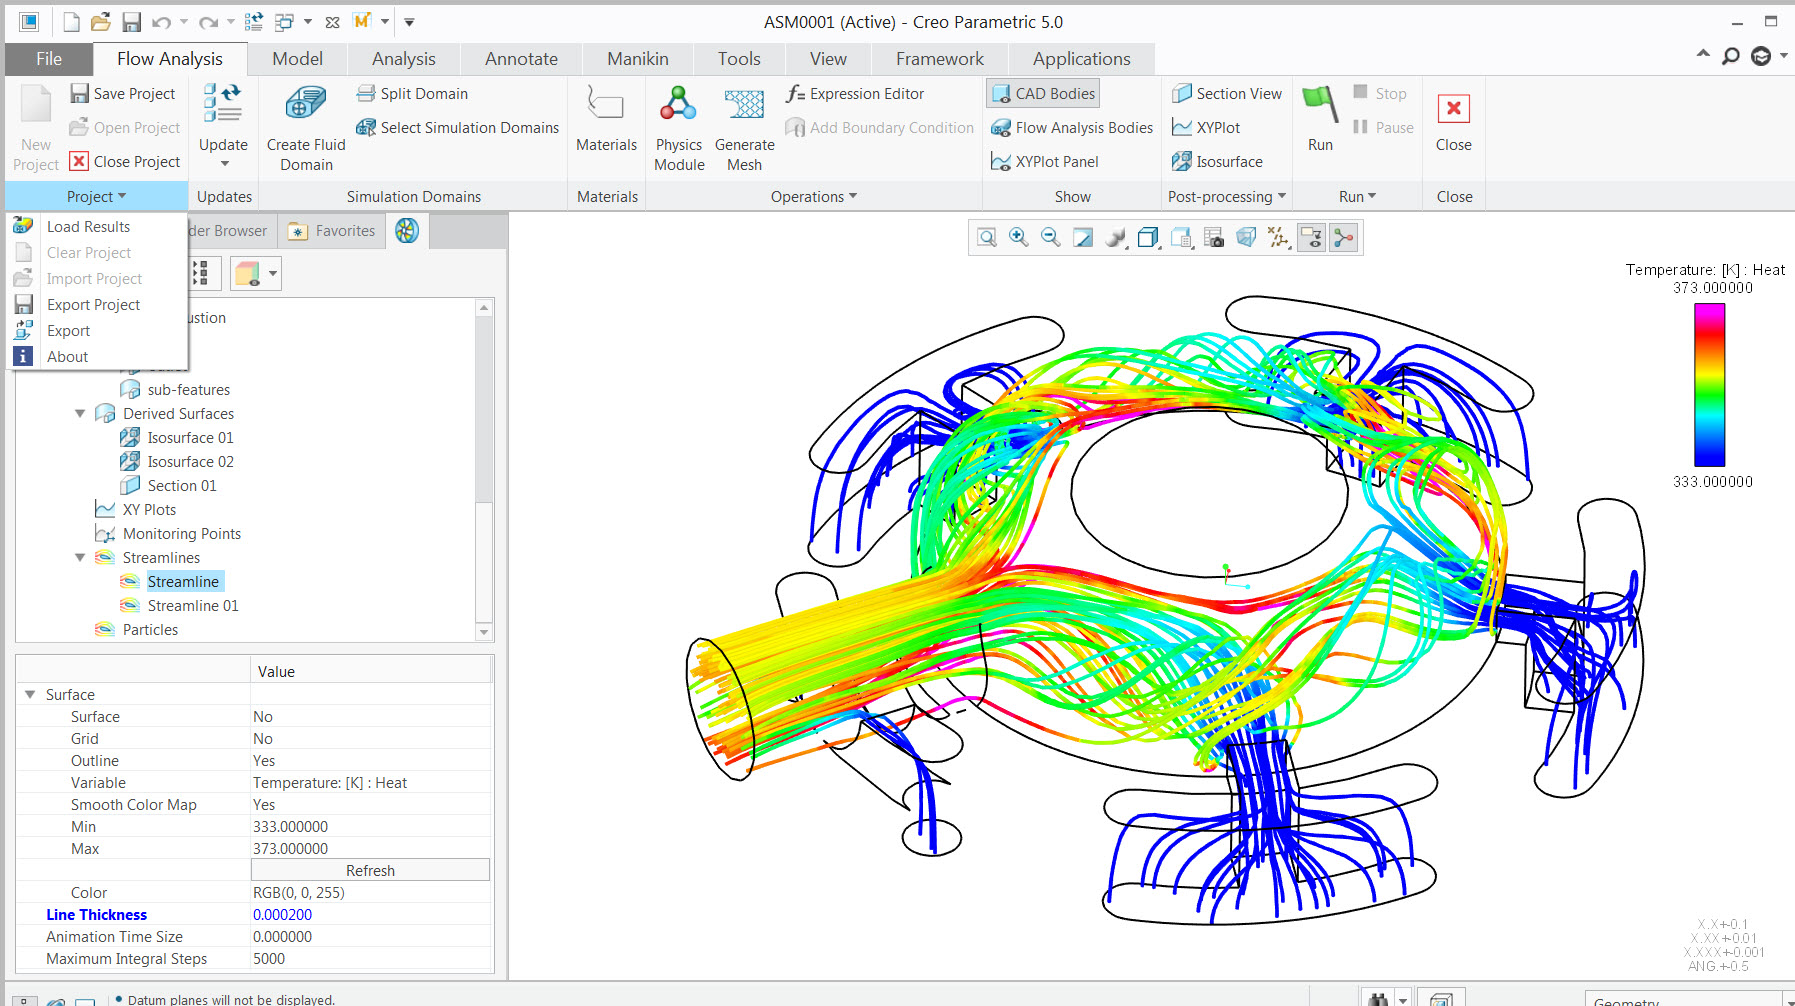
\includegraphics[width=\linewidth]{cylinderhead}
    \caption{I should also note that simulation products are coming into the market aimed at designers who want tools with instantaneous simulation capabilities.}
  \end{figure}
  
  This concludes our discussion on the operating principles of \acrshort{TDLAS} and the physical nature of the gas absorption lines that will be of importance in the rest of this dissertation. Now, we will briefly discuss why \acrshort{TDLAS} is used and what types there are.

  \Acrshort{TDLAS} has several advantages: a high signal-to-noise ratio, a high degree of specificity if a non-interfering region can be found, as is often the case (i.e.\ there exist no nearby absorption lines of gasses that can also be present in the gas cell), and fast measurement compared to other techniques such as non-dispersive gas sensing. A thorough review of different optical measurement techniques can be found in \cite{OpticalGasSensingReview}. %These are of~course desired since the main goal is to build a reliable real-time measurement system (see also \cref{}\todo{link to main goal/questions}).

  Two forms of \acrshort{TDLAS} exist: line scanning and \acrshort{WMS}. In the case of line scanning, the laser is swept over an absorption peak. In the case of \acrshort{WMS}, the input signal is not only swept over the feature, but an additional small-scale sine modulation is applied to the input signal. The frequency of this sine wave is typically much higher than the ramp of triangle that sweeps over the entire absorption feature. 
  
  \subsection{Line Scanning Absorption Spectroscopy}\label{background:line-scanning-absorption-spectroscopy}
  
    The easiest way to determine a gas concentration is by means of a line scanning absorption spectroscopy measurement. The input is a ramping function (or triangle wave) that ideally only ramps the output wavelength while maintaining a constant output power. In practice, the output power is modulated too. This power modulation result in a \acrfull{RAM} at the detector that needs to be removed.
    
    A computer simulation of a direct absorption spectroscopy measurement is depicted. A current ramp around the desired bias current is applied to the input of the laser. The laser emission wavelength will also have this ramp modulation and thus scan over the absorption feature. The light-matter interaction in the gas cell will cause different powers being detected by the photodiode than those emitted by the laser. The resulting photodiode output current will thus depend upon gas properties. An amplifier then amplifies the signal to suitable levels for digital conversion. Finally, the computer processes the data.
    
    Typically, the concentration is extracted using a single point (the minimum due to the absorption peak) or by means of integration of the incident light. Using the law of Beer-Lambert (\cref{background:Beer-Lambert-law}), the concentration is extracted \cite{OpticalGasSensingReview} after subtraction of the \acrshort{RAM}. Since measurements are typically done in ambient conditions, the absorption peak will have an approximate Lorentzian line profile in \cref{background:absorption-coefficient} \cite{spectrochemical-analysis}.
    
    The major advantage of this method is its simplicity. A single ramping (or triangle) function is needed to scan over the feature to find the dip resulting from absorption. Then the concentration is extracted. This simplicity does limit the resolution however. \acrshort{WMS} typically has improved \acrshort{SNR} due to its zero baseline and higher dependence on spectral features \cite{OpticalGasSensingReview}. 

  \subsection{Wavelength Modulation Spectro\-scopy}\label{background:WMS}

    For \acrshort{WMS}, the laser is tuned with a slow and fast varying signal. A fast sinusoid (typically with a frequency of \SIrange{1}{100}{\kilo\hertz}) is superimposed on a low-frequency ramp (or triangle with a typical frequency of \SIrange{1}{100}{\hertz}), the sum of these two signals (and a biasing component) is then fed into the laser to tune the wavelength of the emitted laser line \cite{OSA-freq-int-modulation}.

    Each of these input currents have a specific function. The bias current sets the absorption line over which the ramp (or triangle) modulation scans. The ramp (or triangle) changes the biasing conditions of the laser and the fast sinusoid scans (partially) over the absorption line. In the subsequent, we will refer to this sinusoid as the first order harmonic.
    
    The absorption line cause the transmission function to be non-linear. This will cause formation of different harmonics of the fast sinusoid in the incident light on the photodiode. Higher order harmonics are highly dependent on the spectral shape (as they are caused by the spectral line) and are thus ideal for gas property extraction. These can be detected using \acrfullpl{LIA}. \acrshortpl{LIA} can be seen as narrow band digital filtering structures. 
    
    As we can observe, the bias current set the output power of the wavelength to a mean value of about \SI{0.2915}{\milli\watt}, the ramp scans over the entire absorption line and the sine does so partially. The variation of the first order harmonic amplitude can also be clearly observed in the figure: constant amplitudes near \SI{0.5}{\second} and \SI{0.55}{\second}, but much larger amplitude to the left and right of the maximum absorption and almost zero at the minimum absorption. This is due to the shape of the absorption line. The second order harmonic is not visible here (since it's much smaller). But it can be made visible using \acrshortpl{LIA}.
    
    The main advantage of this technique is improved \acrfull{SNR} due to the usage of \acrshortpl{LIA}. They allow to extract signals near the noise floor. Additionally, by using a high frequency sine (typically at least a \SI{10}{\kilo\hertz}), the system can more easily escape the $1/f$~noise region. Higher order harmonics are also highly dependent on the absorption line, making them good candidates for concentration extraction. While the \acrshort{SNR} can be improved, the extracted harmonics are typically quite weak (and increasingly so for higher order harmonics). The first and/or second order harmonics are usually used. These can for instance be combined to form a ratio. The concentration is extracted based on a mathematical model or simulations. 
    
    Generally the \acrfull{2f} is used because this harmonic has high dependence on gas properties and is stronger than higher order (third, fourth\ldots) harmonics. The first order harmonic may be used for normalisation. This removes laser drift, amplitude modulations and possible vibrations \cite{RiekerDissertation}. Care must be taken however, that the \acrfull{1f} signal does not become zero. This problem can be alleviated by means of \emph{apodized 2f/1f wavelength modulation spectroscopy} \cite{apodized-WMS}. This technique will not be explored further, since we focus on lower gas concentration measurements in this dissertation.
    
    The \acrshort{1f} is not centred around \num{0} because it is already present in the laser output light. However, this component usually does not pass through zero.
    
    The main disadvantage of this technique is that the harmonic amplitudes are usually quite low (especially the second order component.    
    
    \begin{lstlisting}[caption={Some Python code},label={lst:label},language=Python]
from ftplib import FTP, FTP_TLS
from subprocess import Popen, PIPE
import re, os, socket, time


def get_camera_ip(mac="0:13:95:14:6c:c"):
stdout, stderr = Popen(["arp -a | egrep '%s'" % mac], shell=True, stdout=PIPE).communicate()
data = re.findall("\([0-9\.]+\)", stdout.decode("utf-8"))
print(data)
data = data[0][1:-1]
return data


# Check if directory exists (in current location)
def directory_exists(ftp, dir):
filelist = []
ftp.retrlines('LIST',filelist.append)
for f in filelist:
if f.split()[-1] == dir and f.upper().startswith('D'):
return True
return False

def chdir(ftp, dir):
if directory_exists(dir) is False: # (or negate, whatever you prefer for readability)
ftp.mkd(dir)
ftp.cwd(dir)

class SyncFTP:
def __init__(self, mac="0:13:95:14:6c:c"):
ip_camera = socket.gethostbyname("camera-00-13-95-14-6c-0c.local")
#ip_server = socket.gethostbyname("rigel.local")
#ip = get_camera_ip(mac)
self.ftp_camera = FTP(ip_camera)
#self.ftp_server = FTP_TLS(ip_server)

def transfer(self, src, delete=False, dst=""):
dirs = [src]
try:
self.ftp_camera.login(user="anonymous", passwd="")
#self.ftp_server.sendcmd("USER user1")
#self.ftp_server.sendcmd("PASS user1")
while len(dirs) > 0:
d = dirs.pop()
self.ftp_camera.cwd(d)
dir_prefix = self.ftp_camera.pwd()
dir_prefix = dir_prefix.replace(src, ".")
if not os.path.exists(dir_prefix):
os.makedirs(dir_prefix)
lines = []
self.ftp_camera.retrlines('LIST', callback=lines.append)
time.sleep(2)
for line in lines:
args = line.split(" ")
permissions = args[0]
name = args[-1]
if permissions[0] == "d":
dirs.append(self.ftp_camera.pwd() + "/" + name)
else:
target_dir = os.path.join(dst, dir_prefix)
if not os.path.isdir(target_dir):
os.makedirs(target_dir)
self.ftp_camera.retrbinary("RETR %s" % name, open(os.path.join(target_dir, name), "wb").write)
print("Transfer of", name)
if delete:
self.ftp_camera.delete(name)
#self.ftp.rmd(self.ftp.)
finally:
self.ftp_camera.close()


if __name__ == "__main__":
while True:
sftp = SyncFTP()
sftp.transfer(src="/data", delete=True, dst="/mnt") #  dst="/Users/Olivier/"
#time.sleep(10)
  \end{lstlisting}
   
\section{Overview of this Dissertation}\label{background:overview}

  Write the overview here. \lipsum[1]
  
   

\end{document}
